\newpage

\section{Actividad 4: Característica de transferencia de corriente}

\section*{Objetivo}
Se propondrá una práctica de laboratorio que nos permitirá observar sí la relación
entre la $I_C$ e $I_B$ se mantiene constante en diferentes regiones de trabajo del transistor. Esta
relación es la ganancia de corriente ($\beta$).

La simulación a realizar esta dada por el siguiente circuito:

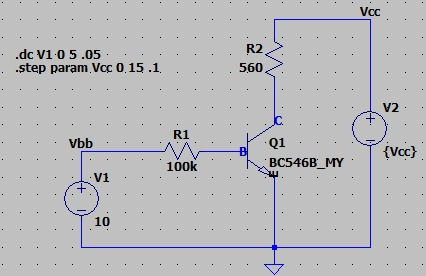
\includegraphics[width=7cm]{./imagenes/Circuito4.jpg}


\subsection{Materiales usados:}

\begin{itemize}
    \item Transistor BC546/7/8/9.
    \item Resistores $R_B = \SI{100}{\kilo\ohm}$, $R_c = \SI{560}{\ohm}$.
    \item Dos fuentes variables de 0V hasta (al menos) 10V.
\end{itemize}

\subsection{Tabla de medición}

\begin{table}[ht]
\resizebox{\columnwidth}{!}{%
\begin{tabular}{|l|l|l|l|}
\hline
\rowcolor[HTML]{FFCC67} 
$I_B\ [\mu A]$ & $I_C\ (@\ V_{CE(inicial)} = 2\,V)$ & $I_C\ (@\ V_{CE(inicial)} = 5\,V)$ & $I_C\ (@\ V_{CE(inicial)} = 8\,V)$ \\ \hline
5  & $1,76 mA$ & $1,85 mA$ & $1,94 mA$ \\ \hline
7  & $2,4 mA$  & $2,52 mA$ & $2,64 mA$ \\ \hline
10 & $3,5 mA$  & $3,67 mA$ & $3,85 mA$ \\ \hline
20 & $6,31 mA$ & $6,63 mA$ & $6,94 mA$ \\ \hline
\end{tabular}%
}
\end{table}

\subsection{Gráficos}

Gráfico $I_C = f(I_B)$ para las diferentes curvas (VCE(inicial) = 2V, 5V y 8V) y el valor de $\beta$ obtenido en cada una de las diferentes curvas.

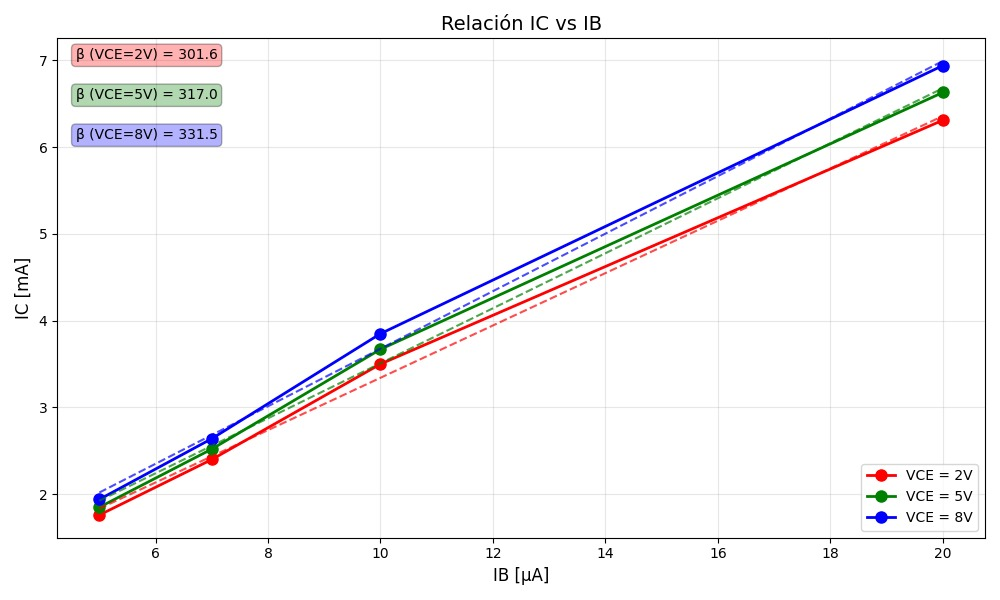
\includegraphics[width=9cm]{./imagenes/Grafico4.jpg}
